% Two-Body Gravity --- technical documentation
% Build:  latexmk -pdf two-body.tex     (see the final section for prerequisites)

\documentclass[11pt,a4paper]{article}

\usepackage[T1]{fontenc}
\usepackage[utf8]{inputenc}
\usepackage{lmodern}
\usepackage[margin=28mm]{geometry}
\usepackage{amsmath}
\usepackage{amssymb}
\usepackage{graphicx}
\usepackage{booktabs}
\usepackage{listings}
\usepackage{xcolor}
\usepackage{microtype}

\definecolor{NavyBlue}{RGB}{20,70,140}
\definecolor{CodeBg}{RGB}{247,247,250}
\definecolor{CodeKw}{RGB}{150,40,120}
\definecolor{CodeCm}{RGB}{100,110,120}
\definecolor{CodeStr}{RGB}{30,110,80}

\usepackage[colorlinks=true,linkcolor=NavyBlue,urlcolor=NavyBlue,
            citecolor=NavyBlue]{hyperref}

\lstdefinelanguage{Rust}{
  keywords={fn,let,mut,pub,struct,impl,for,in,if,else,while,loop,match,return,
            self,Self,const,use,mod,as,true,false,enum,type,where,move,ref},
  sensitive=true,
  comment=[l]{//},
  morecomment=[s]{/*}{*/},
  morestring=[b]",
}

\lstset{
  basicstyle=\ttfamily\small,
  keywordstyle=\color{CodeKw}\bfseries,
  commentstyle=\color{CodeCm}\itshape,
  stringstyle=\color{CodeStr},
  backgroundcolor=\color{CodeBg},
  frame=single,
  rulecolor=\color{black!18},
  framesep=5pt,
  xleftmargin=6pt,
  xrightmargin=6pt,
  breaklines=true,
  showstringspaces=false,
  columns=fullflexible,
  keepspaces=true,
}

% Vector notation used throughout: bold upright for vectors.
\newcommand{\vd}{\mathbf{d}}
\newcommand{\vr}{\mathbf{r}}
\newcommand{\vv}{\mathbf{v}}
\newcommand{\va}{\mathbf{a}}
\newcommand{\vF}{\mathbf{F}}
\newcommand{\ve}{\mathbf{e}}
\newcommand{\vP}{\mathbf{P}}
\newcommand{\vR}{\mathbf{R}}
\newcommand{\vV}{\mathbf{V}}
\newcommand{\dhat}{\hat{\mathbf{d}}}
\newcommand{\dt}{\Delta t}

\title{\textbf{Two-Body Gravity}\\[2pt]
       \large A real-time gravitational simulation in Rust}
\date{}

\begin{document}
\maketitle
\thispagestyle{empty}

\begin{abstract}
\noindent
A real-time simulation of two point masses under mutual Newtonian gravity.
The physics runs in double precision on a fixed timestep, integrated with
velocity Verlet; rendering is immediate-mode OpenGL via
\href{https://macroquad.rs}{macroquad}. This document derives every formula the
program uses, explains why each numerical method was chosen over its
alternatives, and describes how the results are verified.
\end{abstract}

\begin{figure}[htbp]
  \centering
  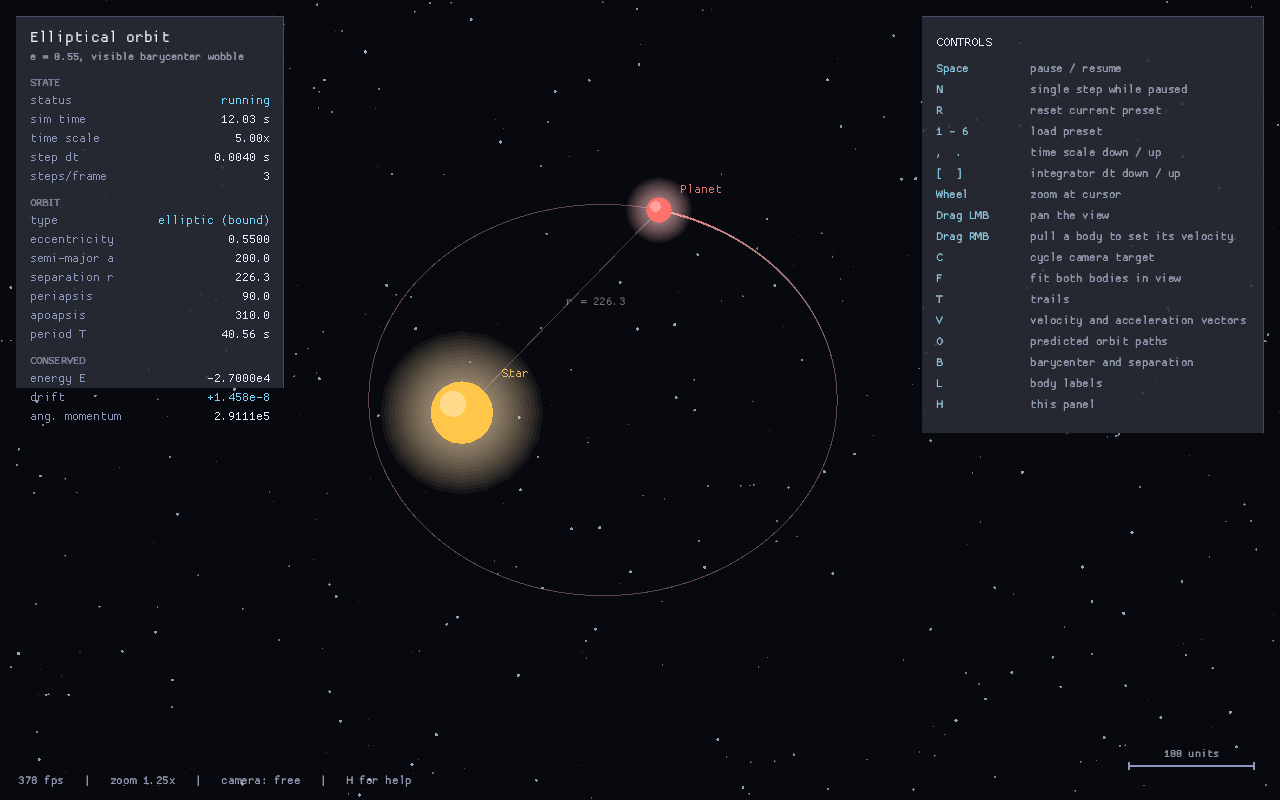
\includegraphics[width=\textwidth]{elliptical.png}
  \caption{The elliptical preset ($e = 0.55$). The panel on the left reports
  orbital elements derived analytically from the instantaneous state vector,
  independently of the integrator that produced it.}
\end{figure}

\tableofcontents
\newpage

%======================================================================
\section{Running the program}

The simulation is a standard Cargo project and needs only a Rust toolchain.
Install one from \url{https://rustup.rs} if you do not have it, then:

\begin{lstlisting}
cargo run --release
\end{lstlisting}

\noindent
The \texttt{--release} flag matters: the debug build is roughly an order of
magnitude slower.

\medskip
\noindent
On Linux, macroquad additionally needs the system OpenGL and X11 development
libraries. On Debian or Ubuntu:

\begin{lstlisting}
sudo apt install libx11-dev libxi-dev libgl1-mesa-dev
\end{lstlisting}

\medskip
\noindent Two optional flags are accepted:

\begin{center}
\begin{tabular}{@{}ll@{}}
\toprule
\textbf{Flag} & \textbf{Effect}\\
\midrule
\texttt{--preset <1--6>}  & start on a given configuration\\
\texttt{--capture <path>} & render a few seconds, write a PNG, exit\\
\bottomrule
\end{tabular}
\end{center}

\noindent
The second exists so the visuals can be checked without a person at the
keyboard, which is how the figures in this document were produced.

%----------------------------------------------------------------------
\subsection{Controls}

\begin{center}
\begin{tabular}{@{}ll@{}}
\toprule
\textbf{Key} & \textbf{Action}\\
\midrule
\texttt{Space}      & pause / resume\\
\texttt{N}          & single step while paused\\
\texttt{R}          & reset the current preset\\
\texttt{1}--\texttt{6} & load a preset\\
\texttt{,} \texttt{.}  & time scale down / up\\
\texttt{[} \texttt{]}  & integrator step size down / up\\
Wheel               & zoom at the cursor\\
Drag LMB            & pan\\
Drag RMB            & pull from a body to set its velocity\\
\texttt{C}          & cycle camera target (free / barycenter / either body)\\
\texttt{F}          & frame the whole orbit\\
\texttt{T V O B L}  & toggle trails, vectors, predicted orbits, barycenter, labels\\
\texttt{P}          & save a screenshot\\
\texttt{H}          & controls panel\\
\texttt{Esc} / \texttt{Q} & quit\\
\bottomrule
\end{tabular}
\end{center}

%----------------------------------------------------------------------
\subsection{Presets}

\begin{enumerate}\itemsep2pt
  \item \textbf{Circular orbit} --- $e = 0$, light satellite.
  \item \textbf{Elliptical orbit} --- $e = 0.55$, with a visible barycenter wobble.
  \item \textbf{Comet} --- $e = 0.9$, a fast periapsis passage.
  \item \textbf{Equal-mass binary} --- two identical bodies on mirrored ellipses.
  \item \textbf{Hyperbolic flyby} --- unbound; deflected once and gone.
  \item \textbf{Radial infall} --- zero angular momentum, straight-line collapse.
\end{enumerate}

%======================================================================
\section{The physical model}
\label{sec:model}

Two point masses $m_0$ and $m_1$ at positions $\vr_0$ and $\vr_1$. Everything
below is built from the separation vector between them:
\[
  \vd = \vr_1 - \vr_0 .
\]

\subsection{Deriving the acceleration}

\paragraph{Step 1 --- Newton's law of gravitation,} in the form everyone learns
it. Note that it gives only a \emph{magnitude}:
\[
  |\vF| = \frac{G\,m_0\,m_1}{r^2},
  \qquad r = |\vd| .
\]

\paragraph{Step 2 --- attach a direction.} Force is a vector, so the magnitude
needs a unit vector to point it. Body 0 is pulled \emph{toward} body 1, and
since $\vd$ points from 0 to 1, that direction is $\dhat = \vd/|\vd|$:
\[
  \vF_0 \;=\; \frac{G\,m_0\,m_1}{|\vd|^2}\,\dhat
        \;=\; \frac{G\,m_0\,m_1}{|\vd|^2}\cdot\frac{\vd}{|\vd|}
        \;=\; \frac{G\,m_0\,m_1\,\vd}{|\vd|^3} .
\]

\paragraph{Step 3 --- Newton's second law,} $\vF = m\va$, so divide through by
$m_0$:
\begin{align}
  \va_0 &= \phantom{-}\frac{G\,m_1\,\vd}{|\vd|^3}, \label{eq:a0}\\[2pt]
  \va_1 &= -\frac{G\,m_0\,\vd}{|\vd|^3}. \label{eq:a1}
\end{align}

Equations \eqref{eq:a0} and \eqref{eq:a1} are the entire physics. The rest of
the simulation is machinery for integrating them accurately and drawing the
result.

\subsection{The cube is not an inverse-cube force}

Gravity here is still $1/r^2$. The exponent reads 3 only because $\vd$ in the
numerator is \emph{un-normalized} --- it carries a factor of $|\vd|$ in its own
length. Splitting it back apart:
\[
  \frac{\vd}{|\vd|^{3}}
  \;=\;
  \underbrace{\frac{1}{|\vd|^{2}}}_{\text{magnitude}}
  \;\cdot\;
  \underbrace{\vphantom{\frac{1}{|\vd|^{2}}}\;\dhat\;}_{\text{direction}}
\]

Fusing the two is a numerical convenience: normalizing $\vd$ first and then
scaling would need a second division by $|\vd|$. The code computes $|\vd|^3$ as
\texttt{r2 * r2.sqrt()}, that is $|\vd|^2\cdot|\vd|$, for one square root in
total.

Dimensions confirm it is an acceleration. With
$[G] = \mathrm{m^3\,kg^{-1}\,s^{-2}}$:
\[
  \frac{\mathrm{m^{3}\,kg^{-1}\,s^{-2}} \cdot \mathrm{kg} \cdot \mathrm{m}}
       {\mathrm{m^{3}}}
  \;=\; \mathrm{m\,s^{-2}} .
\]
Leaving $|\vd|^2$ in the denominator would yield $\mathrm{m^2\,s^{-2}}$, which
is not an acceleration --- the cube is what makes the units come out right.

\subsection{Why \texorpdfstring{$m_0$}{m0} cancels}

The \emph{force} on body 0 depends on both masses, but its \emph{acceleration}
depends only on $m_1$, the mass of the other body. The $m_0$ in the
gravitational law is cancelled by the $m_0$ in $\vF = m_0\va$.

That cancellation is the equivalence principle --- how strongly a body is pulled
and how strongly it resists being pulled are the same number, so heavy and light
objects fall identically. It is visible directly in
\texttt{System::compute\_accelerations}, where each body's acceleration is
scaled by the \emph{other} body's mass:

\begin{lstlisting}[language=Rust]
self.bodies[0].acc = d * (self.g * m1 * inv_r3);   // uses the OTHER mass
self.bodies[1].acc = d * (-self.g * m0 * inv_r3);
\end{lstlisting}

The only difference between the two lines is the sign. Both bodies accelerate
along the same axis $\vd$ in opposite directions, which is Newton's third law,
and why the pair's total momentum never changes.

\subsection{Why the state is stored as vectors}

A two-body orbit is planar, so it could be described with scalars --- a radius
and an angle, or a set of orbital elements --- and some simulations do exactly
that. This one keeps position, velocity and acceleration as \texttt{V2} vectors
and integrates the ODE directly. The reasons are concrete:

\begin{itemize}\itemsep3pt
  \item \textbf{A magnitude alone is not a force.} $G m_0 m_1 / r^2$ says how
    hard, never which way. The direction has to be reintroduced somehow;
    $\vd/|\vd|^3$ carries both at once and keeps the expression in a single term.
  \item \textbf{No trigonometry in the inner loop.} A polar formulation needs
    $\operatorname{atan2}$, $\sin$ and $\cos$ every step. The vector form needs
    one square root and a handful of multiplies, and it never has to unwrap an
    angle across the $2\pi$ boundary.
  \item \textbf{No special cases at the degenerate configurations.} In polar
    coordinates a radial free-fall has $\dot r$ finite but $\dot\theta$
    undefined, and angular formulations need a branch to survive it. Preset 6
    does exactly this, and the vector code runs it with no special handling:
    $\vd$ simply shrinks along a fixed direction. (The separate problem of
    $|\vd| \to 0$ blowing up the force is what softening in
    Section~\ref{sec:softening} addresses; that one is real, and no choice of
    coordinates avoids it.)
  \item \textbf{The orbit's orientation is an output, not a coordinate choice.}
    Nothing in the integrator knows where periapsis is or which way the orbit is
    tilted. The argument of periapsis $\omega$ is \emph{derived} in
    Section~\ref{sec:elements} from the state, which is what makes those
    elements an independent check on the integrator rather than an assumption
    fed into it.
  \item \textbf{Forces superpose as vectors.} Adding a third body means summing
    $\vd/|\vd|^3$ terms over pairs; the loop body does not change. Scalar
    magnitudes cannot be summed without reintroducing direction anyway.
  \item \textbf{The integrator is agnostic.} Velocity Verlet
    (Section~\ref{sec:verlet}) is written once in terms of $+$ and
    multiplication by a scalar, and applies unchanged to position, velocity and
    acceleration because all three are the same type. That is why
    \texttt{src/vec2.rs} implements the operator traits --- the physics reads
    like the equations above.
\end{itemize}

The cost is that \texttt{V2} is a hand-rolled \texttt{f64} type rather than the
\texttt{f32} \texttt{Vec2} macroquad provides. Orbits accumulate error over
millions of steps, and \texttt{f32}'s ${\sim}7$ decimal digits are not enough.
The narrowing to \texttt{f32} happens only at the drawing boundary, in
\texttt{Camera::world\_to\_screen} --- so precision is spent on the trajectory
and merely rounded off on the way to a pixel.

The whole system state is six numbers per body: position, velocity, and the
cached acceleration. There is no force accumulator, no collision resolution, and
no drag.

%======================================================================
\section{Softening}
\label{sec:softening}

A literal $1/r^2$ force diverges as the separation goes to zero. The
radial-infall preset drives the bodies straight through each other, so this is
not hypothetical. The fix is \textbf{Plummer softening}: replace the distance
with a value that has a floor,
\[
  |\vd|^{3} \;\longrightarrow\; \bigl(|\vd|^{2} + \varepsilon^{2}\bigr)^{3/2},
\]
with $\varepsilon = 0.5$ world units by default. The important property is that
this softened force is still the exact gradient of a softened \emph{potential},
\[
  U = -\frac{G\,m_0\,m_1}{\sqrt{|\vd|^{2} + \varepsilon^{2}}},
  \qquad
  \vF_0 = -\nabla_{\vr_0} U ,
\]
so the softened system remains perfectly Hamiltonian and energy conservation
stays meaningful. The simulation is exactly integrating a slightly different,
non-singular force law rather than approximating the real one badly.

This consistency is not optional. Soften the force but not the potential and the
force stops being any potential's gradient, at which point the conserved energy
reported in Section~\ref{sec:conserved} would be measuring nothing.

At the separations the presets use the correction is negligible. For
$r = 220$ and $\varepsilon = 0.5$,
\[
  \left(1 + \frac{\varepsilon^{2}}{r^{2}}\right)^{3/2}
  = 1 + 7.7\times10^{-6},
\]
under ten parts per million.

%======================================================================
\section{Integration: velocity Verlet}
\label{sec:verlet}

Given accelerations, the integrator advances the state by $\dt$:
\begin{align}
  \vr(t+\dt) &= \vr(t) + \vv(t)\,\dt + \tfrac12\,\va(t)\,\dt^{2}
    &&\text{drift}\label{eq:vv1}\\
  \va(t+\dt) &= \va\bigl(\vr(t+\dt)\bigr)
    &&\text{recompute forces}\label{eq:vv2}\\
  \vv(t+\dt) &= \vv(t) + \tfrac12\bigl[\va(t) + \va(t+\dt)\bigr]\dt
    &&\text{kick}\label{eq:vv3}
\end{align}

The drift step \eqref{eq:vv1} uses the \emph{old} acceleration; the kick step
\eqref{eq:vv3} averages old and new. That averaging is the entire trick, and it is why the old
acceleration is cached on each \texttt{Body} rather than recomputed. The cost is
one force evaluation per step.

\subsection{Why this integrator and not RK4}

Velocity Verlet is \emph{symplectic}: it exactly conserves a ``shadow''
Hamiltonian that differs from the true one by $O(\dt^{2})$. The practical
consequence is that its energy error is \textbf{bounded and oscillatory} rather
than accumulating.

\begin{center}
\begin{tabular}{@{}lcl@{}}
\toprule
\textbf{Integrator} & \textbf{Order} & \textbf{Energy behaviour}\\
\midrule
Explicit Euler        & 1 & pumps energy in; the orbit spirals outward\\
RK4                   & 4 & very accurate per step, but slowly bleeds energy\\
\textbf{Velocity Verlet} & 2 & error oscillates in a fixed band; the orbit closes\\
\bottomrule
\end{tabular}
\end{center}

RK4 has the better local truncation error and the worse long-run behaviour. For
a simulation meant to run for millions of steps, bounded error beats small
error. Verlet is also time-reversible: stepping forward then backward by $\dt$
returns to the starting state up to rounding.

\subsection{The drift readout}

The heads-up display reports
\[
  \text{drift} = \frac{E - E_0}{|E_0|},
\]
which is the live evidence for the paragraph above. It reads
$+5.4\times10^{-15}$ on the circular preset --- the \texttt{f64} noise floor ---
and between $10^{-9}$ and $10^{-8}$ on the eccentric ones, and it does not trend
upward over time. A growing value means $\dt$ is too large for the current
periapsis speed; \texttt{[} shrinks it.

%======================================================================
\section{Decoupling physics from the frame rate}

Stepping by the frame time would make the trajectory depend on rendering speed,
so results would differ between machines and change when the window is dragged.
Instead the simulation banks elapsed real time and spends it in fixed $\dt$
chunks:

\begin{lstlisting}[language=Rust]
accumulator += min(frame_time, 0.05) * time_scale;
while accumulator >= dt && substeps < 6000 {
    step(dt);
    accumulator -= dt;
}
\end{lstlisting}

Three details matter:

\begin{itemize}\itemsep3pt
  \item \texttt{min(frame\_time, 0.05)} --- clamping the frame delta stops a
    stall (window drag, first frame, a breakpoint) from queuing an unbounded
    backlog of physics.
  \item \texttt{substeps < 6000} --- capping the inner loop makes an extreme
    time scale degrade into slow motion instead of freezing the window.
  \item \texttt{time\_scale} multiplies simulated time per real second; it never
    touches $\dt$, so speeding up the view cannot change the trajectory. Only
    \texttt{[} and \texttt{]} change $\dt$, and those are the accuracy control.
\end{itemize}

Defaults are $\dt = 0.004\,\mathrm{s}$ and a time scale of $5$.

%======================================================================
\section{Conserved quantities}
\label{sec:conserved}

The panel tracks the quantities the true dynamics must preserve. They are
computed from the raw state, independently of the integrator, so they act as a
running self-check.
\begin{align*}
  M    &= m_0 + m_1 &&\text{total mass}\\
  \vR  &= \frac{m_0\vr_0 + m_1\vr_1}{M} &&\text{barycenter}\\
  \vP  &= m_0\vv_0 + m_1\vv_1 &&\text{linear momentum}\\
  K    &= \sum_i \tfrac12 m_i |\vv_i|^{2} &&\text{kinetic energy}\\
  U    &= -\frac{G m_0 m_1}{\sqrt{|\vd|^{2}+\varepsilon^{2}}} &&\text{potential energy}\\
  E    &= K + U &&\text{total energy}\\
  L    &= \sum_i m_i \,(\vr_i - \vR) \times (\vv_i - \vV) &&\text{angular momentum}
\end{align*}

$L$ is taken about the barycenter and in the barycenter's own velocity frame
($\vV = \vP/M$), so it stays invariant even if the pair is drifting. In two
dimensions the cross product is the scalar $x_1 y_2 - y_1 x_2$.

Every preset is passed through \texttt{zero\_momentum()} at load, which subtracts
$\vR$ from the positions and $\vV$ from the velocities. This puts the pair in the
center-of-mass frame with $\vP = 0$ and $\vR = 0$, so the barycenter is a fixed
point and the orbits stay on screen. Setting a velocity by hand with right-drag
breaks that, which is why the camera can follow the barycenter.

%======================================================================
\section{Reduction to relative motion}
\label{sec:relative}

Subtracting the two accelerations of Section~\ref{sec:model} collapses the pair
into a single body:
\[
  \ddot{\vd} = \va_1 - \va_0
             = -\frac{G(m_0+m_1)\,\vd}{|\vd|^{3}}
             = -\frac{\mu\,\vd}{|\vd|^{3}},
  \qquad \mu = G M .
\]

This is the one-body Kepler problem with \textbf{gravitational parameter} $\mu$.
It is exactly solvable, which is why the panel can show real orbital elements
rather than measured estimates. The individual positions come back from $\vd$
and the barycenter by mass fraction:
\begin{align}
  \vr_0 &= \vR - \frac{m_1}{M}\,\vd, \label{eq:split0}\\
  \vr_1 &= \vR + \frac{m_0}{M}\,\vd. \label{eq:split1}
\end{align}

Each body traces the \emph{same conic}, scaled by the other body's mass fraction
and rotated $180^\circ$ from its partner. That is why the equal-mass binary
shows two identical interlocking ellipses, while a star with a light planet
shows a huge planetary ellipse and a barely-visible stellar wobble.

%======================================================================
\section{Orbital elements from the state vector}
\label{sec:elements}

The module \texttt{src/orbit.rs} derives the full element set analytically from
the instantaneous relative position $\vd$ and velocity $\vv$, with $r = |\vd|$.
No softening is applied here: these are the elements of the ideal Kepler orbit.
\begin{align*}
  \xi   &= \frac{|\vv|^{2}}{2} - \frac{\mu}{r} &&\text{specific orbital energy}\\
  h     &= \vd \times \vv &&\text{specific angular momentum}\\
  \ve   &= \frac{\bigl(|\vv|^{2} - \mu/r\bigr)\vd - (\vd\cdot\vv)\,\vv}{\mu}
          &&\text{eccentricity vector}\\
  e     &= |\ve| &&\text{eccentricity}\\
  a     &= -\frac{\mu}{2\xi} &&\text{semi-major axis}\\
  r_p   &= a(1-e), \qquad r_a = a(1+e) &&\text{periapsis, apoapsis}\\
  T     &= 2\pi\sqrt{a^{3}/\mu} &&\text{period (Kepler's third law)}\\
  \omega &= \operatorname{atan2}(e_y,\,e_x) &&\text{argument of periapsis}
\end{align*}

The symbol $\xi$ is used for specific orbital energy rather than the $\epsilon$
many texts use, because $\varepsilon$ is already the softening length of
Section~\ref{sec:softening}.

\subsection{The eccentricity vector}

$\ve$ is the \textbf{Laplace--Runge--Lenz} vector. It is a conserved vector
unique to the inverse-square force: it points from the focus toward periapsis
and its length is the eccentricity, so one expression yields both the shape and
the orientation of the orbit.

\subsection{Classification is by energy, not eccentricity}

\[
  \xi < 0 \;\Rightarrow\; \text{elliptic (bound)},\qquad
  \xi \approx 0 \;\Rightarrow\; \text{parabolic},\qquad
  \xi > 0 \;\Rightarrow\; \text{hyperbolic (escape)} .
\]

This distinction is not pedantic. A radial free-fall (preset 6) has $h = 0$, and
$\ve$ reduces to $-\dhat$, so $e = 1$ exactly --- eccentricity alone would call
it parabolic. Its energy is plainly negative, and the energy test correctly
reports a bound, degenerate ellipse with $r_p = 0$ and $r_a$ equal to the drop
distance. The panel shows exactly that: $e = 1.0000$, apoapsis $520.0$,
$L = 0$.

For the true parabolic case $a$ diverges, so the periapsis falls back to
$r_p = h^{2}/(2\mu)$, and apoapsis and period are reported as undefined.

%======================================================================
\section{Drawing the predicted orbit}

The ghost path is the conic in polar form about the focus,
\[
  r(\nu) = \frac{p}{1 + e\cos\nu},
  \qquad p = a\,(1-e^{2}),
\]
where $\nu$ is the true anomaly, measured from periapsis, and $p$ is the
semi-latus rectum. Sweeping $\nu$ symmetrically about zero and rotating by
$\omega$ gives the curve; the sweep direction follows the sign of $h$ so the
drawn path runs the way the body actually travels. Each sampled point is then
mapped to both bodies through the mass fractions \eqref{eq:split0} and
\eqref{eq:split1}.

Two degenerate cases are handled explicitly:

\begin{itemize}\itemsep3pt
  \item \textbf{Hyperbola.} $r$ diverges at the asymptote, where
    $\cos\nu = -1/e$. The sweep stops at $0.985\arccos(-1/e)$, just inside it,
    so the branch is drawn without shooting off to infinity.
  \item \textbf{Radial orbit.} $e = 1$ gives $p = a(1-e^{2}) = 0$, and the
    function returns an empty path. This is correct: the trajectory is a line
    segment, not a conic with area, so nothing is drawn.
\end{itemize}

%======================================================================
\section{Building the initial conditions}

Presets are specified the way an astronomer would state them --- masses,
semi-major axis, eccentricity --- and \texttt{kepler\_pair} converts that into
state vectors. Bodies start at \textbf{apoapsis}, $r = a(1+e)$, with the speed
given by the \textbf{vis-viva} equation:
\[
  v^{2} = \mu\left(\frac{2}{r} - \frac{1}{a}\right).
\]

At apoapsis the velocity is perpendicular to the separation, so the relative
state is $\vd = (r, 0)$ and $\vv = (0, v)$. Splitting about the barycenter, each
body receives the \emph{other} body's mass fraction:
\[
  \vr_0 = -\frac{m_1}{M}\vd, \quad \vv_0 = -\frac{m_1}{M}\vv,
  \qquad
  \vr_1 = +\frac{m_0}{M}\vd, \quad \vv_1 = +\frac{m_0}{M}\vv,
\]
which yields $\vP = 0$ and $\vR = 0$ by construction.

\subsection*{Worked example (preset 1)}

With $m_0 = 1000$, $m_1 = 8$, $a = 220$, $e = 0$:
\begin{align*}
  \mu &= 200 \times 1008 = 201\,600,\\
  v   &= \sqrt{\mu/a} = \sqrt{916.36} = 30.27 \ \text{world units/s},\\
  T   &= 2\pi\sqrt{220^{3}/201\,600} = 45.66\ \mathrm{s}.
\end{align*}

The panel reads $T = 45.66\,\mathrm{s}$ --- the same closed form, so that
agreement only confirms the setup. The stronger check is that the
\emph{integrated} orbit returns to its starting point after exactly that much
simulated time, which is what the test
\texttt{body\_returns\_to\_start\_after\_one\_period} asserts.

%======================================================================
\section{Units}

Units are arbitrary but internally consistent, with $G = 200$ chosen so a
typical orbit spans a few hundred world units and completes in tens of seconds
--- fast enough to watch, large enough to avoid \texttt{f32} rendering
artifacts. Body draw radius follows constant density,
\[
  R = 2.6 \, m^{1/3},
\]
so mass differences read as size differences without a heavy body swamping the
view.

%======================================================================
\section{Rendering}

Drawing is a pure function of state; nothing in \texttt{src/render.rs} mutates
the simulation.

\paragraph{Camera.} World space is $y$-up and metric, screen space is $y$-down
and in pixels, with $z$ the zoom in pixels per world unit:
\begin{align*}
  x_s &= \frac{W}{2} + (p_x - c_x)\,z,\\
  y_s &= \frac{H}{2} - (p_y - c_y)\,z.
\end{align*}

Zooming at the cursor converts the cursor to world space before and after the
zoom change and shifts the center by the difference, so the point under the
mouse stays put. Camera tracking uses framerate-independent exponential
smoothing,
\[
  c \;\mathrel{+}=\; (\text{target} - c)\bigl(1 - e^{-12\,\dt}\bigr),
\]
which keeps a fast orbit from jittering the view. \texttt{F} frames the whole
predicted orbit --- not just the current separation, which would let a light
body swing off screen half a period later --- and accounts for the width of the
panels so the orbit is not centered underneath one.

\paragraph{Trails.} Sampled by distance rather than by time: a point is appended
once the body has moved $1.2$ world units, capped at $3000$ points. Sampling per
frame would make trail length depend on frame rate and time scale. Alpha ramps
as $(i/n)^{1.4}$ from tail to head.

\paragraph{Bodies.} The glow is 14 concentric discs out to $2.6\times$ the
radius, each at alpha $0.028$, summing to
$1 - 0.972^{14} \approx 33\%$ opacity at the core. Many faint layers integrate
into a smooth falloff; a few strong ones would band into visible rings.

\paragraph{Vectors.} Velocity and acceleration arrows are each normalized to the
larger of the two bodies, so the pair stays comparable at any zoom and never
overruns the screen.

%======================================================================
\section{Source layout}

\begin{center}
\begin{tabular}{@{}ll@{}}
\toprule
\textbf{File} & \textbf{Contents}\\
\midrule
\texttt{src/vec2.rs}    & \texttt{f64} 2D vector\\
\texttt{src/physics.rs} & bodies, forces, the Verlet step, conserved quantities\\
\texttt{src/orbit.rs}   & Keplerian elements and the predicted conic\\
\texttt{src/presets.rs} & starting configurations\\
\texttt{src/camera.rs}  & world/screen mapping, pan, zoom, framing\\
\texttt{src/render.rs}  & all drawing\\
\texttt{src/main.rs}    & input, the fixed-step loop, wiring\\
\bottomrule
\end{tabular}
\end{center}

%======================================================================
\section{Tests}

\begin{lstlisting}
cargo test --release
\end{lstlisting}

\noindent The suite checks the physics, not the rendering:

\begin{center}
\begin{tabular}{@{}ll@{}}
\toprule
\textbf{Test} & \textbf{Asserts}\\
\midrule
\texttt{circular\_orbit\_keeps\_its\_radius}
  & radius holds to $10^{-3}$ over 200\,000 steps\\
\texttt{verlet\_does\_not\_drain\_energy}
  & drift $< 10^{-4}$ on an $e=0.8$ orbit over 400\,s\\
\texttt{body\_returns\_to\_start\_after\_one\_period}
  & position closes to $10^{-3}$ after exactly $T$\\
\texttt{barycenter\_and\_momentum\_stay\_put}
  & $\vP$ and $\vR$ remain zero\\
\texttt{elements\_recover\_the\_construction\_parameters}
  & derived $e$ and $a$ match the preset inputs\\
\texttt{elements\_classify\_an\_unbound\_orbit}
  & flyby reports hyperbolic, $e>1$, no period\\
\texttt{softening\_survives\_a\_head\_on\_collapse}
  & radial infall stays finite through contact\\
\bottomrule
\end{tabular}
\end{center}

The period test is the strongest of these: it closes the loop between the
integrator (Section~\ref{sec:verlet}) and the analytic elements
(Section~\ref{sec:elements}), which are computed by completely separate code. If
either were wrong, they would disagree.

%======================================================================
\section{Building this document}
\label{sec:building}

\subsection{Prerequisites}

The document uses only standard packages --- \texttt{amsmath}, \texttt{amssymb},
\texttt{geometry}, \texttt{graphicx}, \texttt{booktabs}, \texttt{listings},
\texttt{xcolor}, \texttt{hyperref}, \texttt{microtype} and \texttt{lmodern} ---
so any reasonably complete \TeX{} installation will do.

\begin{center}
\begin{tabular}{@{}ll@{}}
\toprule
\textbf{Platform} & \textbf{Install}\\
\midrule
Debian / Ubuntu & \texttt{sudo apt install texlive-latex-recommended} \\
                & \texttt{\ \ texlive-latex-extra texlive-fonts-recommended latexmk}\\
Fedora          & \texttt{sudo dnf install texlive-scheme-medium latexmk}\\
Arch            & \texttt{sudo pacman -S texlive-basic texlive-latexrecommended}\\
                & \texttt{\ \ texlive-latexextra}\\
macOS           & \texttt{brew install --cask mactex-no-gui}\\
Windows         & MiKTeX (\url{https://miktex.org}) or TeX Live\\
\bottomrule
\end{tabular}
\end{center}

\medskip
\noindent
A lighter alternative is \textbf{Tectonic}, a single self-contained binary that
downloads only the packages a document actually needs:

\begin{lstlisting}
cargo install tectonic          # or: brew install tectonic
\end{lstlisting}

\subsection{Generating the PDF}

From the \texttt{docs/} directory:

\begin{lstlisting}
latexmk -pdf two-body.tex       # recommended: reruns as needed for the ToC
\end{lstlisting}

\noindent Equivalent alternatives:

\begin{lstlisting}
tectonic two-body.tex           # one command, no latexmk needed

pdflatex two-body.tex           # plain pdflatex: run TWICE, so that the
pdflatex two-body.tex           # table of contents and cross-references resolve
\end{lstlisting}

\noindent
All three write \texttt{two-body.pdf} beside the source. A \texttt{Makefile} is
provided, so \texttt{make} in \texttt{docs/} does the same thing and
\texttt{make clean} removes the intermediate \texttt{.aux}, \texttt{.log},
\texttt{.out} and \texttt{.toc} files.

\medskip
\noindent
The figure \texttt{elliptical.png} must be present in the same directory. It is
committed alongside this source, and can be regenerated at any time with:

\begin{lstlisting}
cargo run --release -- --capture docs/elliptical.png --preset 2
\end{lstlisting}

\end{document}
